%% Section 3: Modeling the AR-DeC Pedagogical Scenario with UML
\section{Modeling the AR-DeC Pedagogical Scenario with UML: A Methodological Approach}
\label{sec:modeling}

Having established the theoretical foundations that underpin AR-DeC---spanning mobile AR in education, vocabulary acquisition theory, intelligent tutoring, gamification, and UML-based pedagogical modeling---we now shift from theory to formalization. The goal of this section is to translate the pedagogical design intent articulated in \Cref{sec:theoretical} into a rigorous, implementation-ready specification using the Unified Modeling Language. UML serves here not merely as a documentation tool but as an \emph{instructional design instrument}: each diagram encodes specific pedagogical decisions, ensuring that the resulting software architecture faithfully reflects the educational objectives~\cite{Booch2005,Ouariach2026}. We adopt two complementary perspectives---a \emph{static view} that captures the structural organization of the system (what entities exist, what they know, and how they relate) and a \emph{dynamic view} that models the behavioral aspects (how the system evolves over time in response to learner interactions). Together, these four diagrams---class, use case, activity, and sequence---provide a complete specification of the AR-DeC pedagogical scenario.

%%% ===================================================================
\subsection{Static View}
\label{sec:static}

The static view describes the enduring structure of the AR-DeC system: the classes that comprise it, the relationships that bind them, and the use cases that define the system boundary. We begin with the class diagram, which constitutes the architectural backbone, and then present the use case diagram, which delineates each actor's functional scope.

%%% -------------------------------------------------------------------
\subsubsection{Class Diagram}
\label{sec:classdiagram}

The class diagram presented in \Cref{fig:classdiagram} constitutes the structural foundation of the AR-DeC pedagogical scenario. It specifies fifteen classes organized into five functional groups---\emph{Core Actors}, \emph{Learning Content}, \emph{Student Modeling}, \emph{AI \& AR}, and \emph{Gamification}---each encapsulating a coherent set of responsibilities. This decomposition reflects a deliberate design strategy: by isolating concerns along pedagogical rather than purely technical boundaries, we ensure that every class can be traced back to a specific educational requirement~\cite{Rumbaugh2004,Ouariach2025}. The five groups mirror the five pillars of the AR-DeC system: the human actors who participate in the learning process, the content that is learned, the models that track what has been learned, the intelligent and immersive engines that deliver content, and the motivational mechanics that sustain engagement.

\begin{landscape}
\begin{figure}[htbp]
\centering
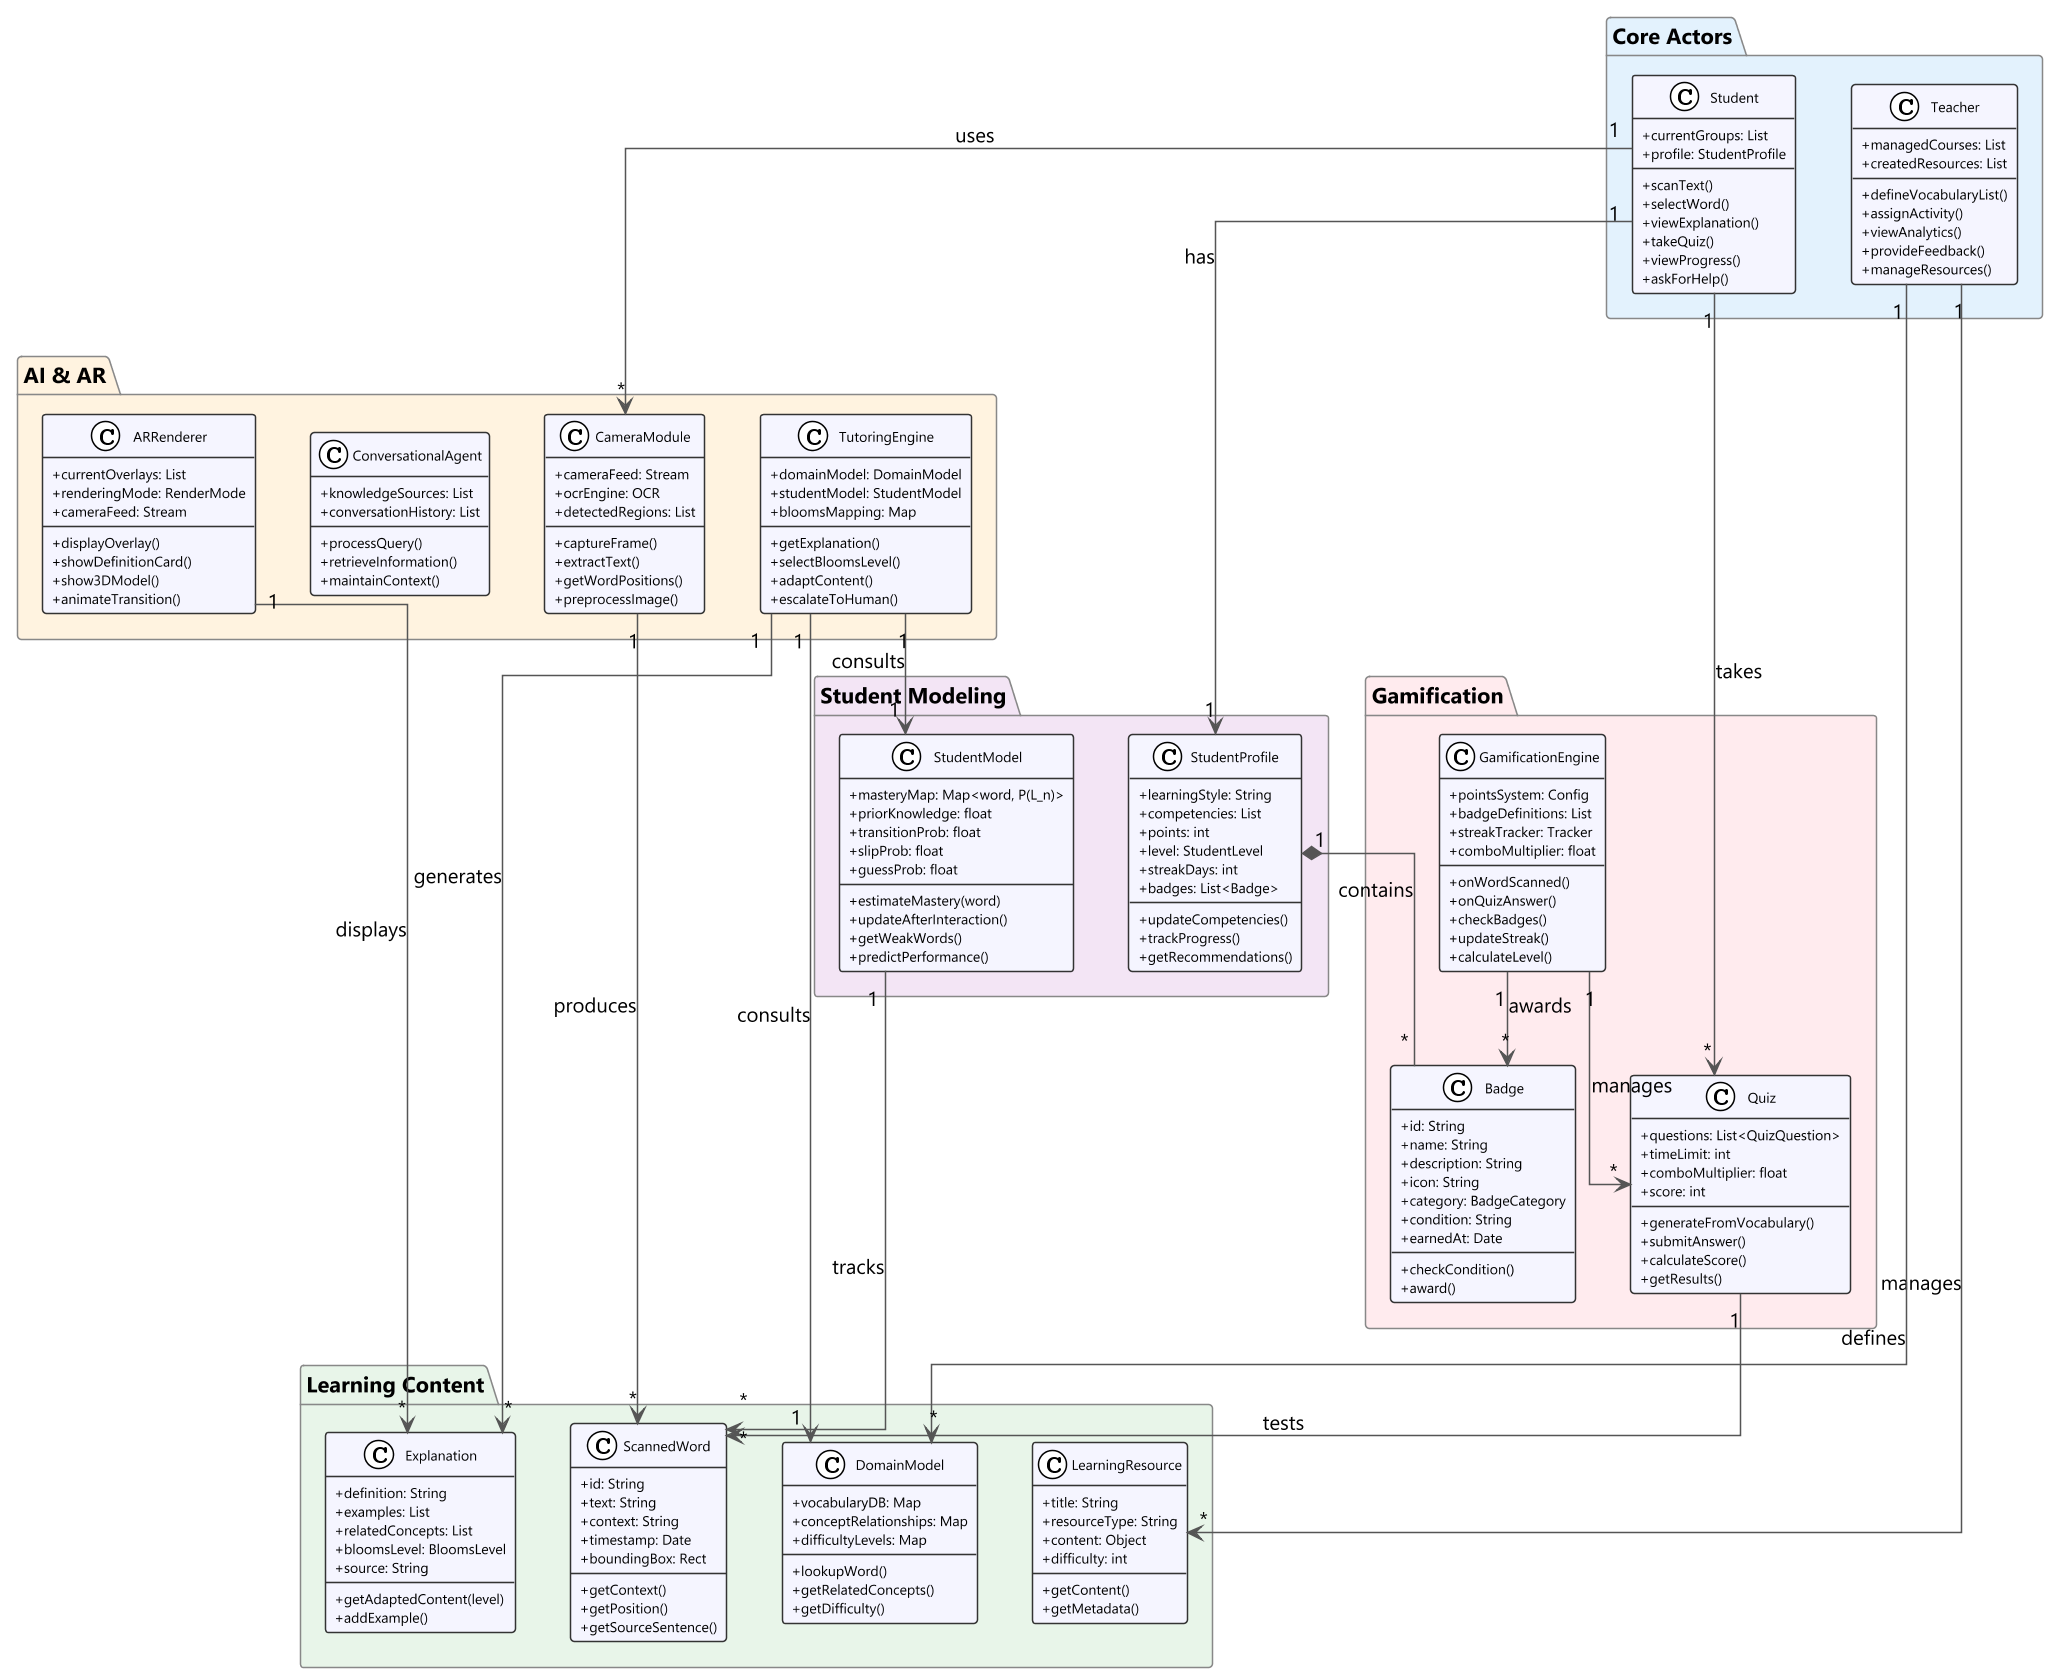
\includegraphics[width=\linewidth,height=0.85\textheight,keepaspectratio]{images/class-diagram.png}
\caption{Class diagram of the AR-DeC pedagogical scenario.}
\label{fig:classdiagram}
\end{figure}
\end{landscape}

We now describe each class in detail, articulating both its pedagogical rationale and its indispensability within the overall architecture.

\bigskip
\noindent\textbf{Group 1: Core Actors}

\medskip
\textbf{Student}
\begin{itemize}
\item \textit{Rationale and Contribution:} The \texttt{Student} class represents the primary user of the AR-DeC system. It maintains references to the groups in which the learner participates (\texttt{currentGroups}) and an associated \texttt{StudentProfile} object that captures the learner's evolving characteristics. Its methods---\texttt{scanText()}, \texttt{selectWord()}, \texttt{viewExplanation()}, \texttt{takeQuiz()}, \texttt{viewProgress()}, and \texttt{askForHelp()}---encode the complete repertoire of learner-initiated interactions, from the initial scanning of a textbook page through vocabulary exploration, assessment, and help-seeking.
\item \textit{Indispensability:} All functionalities of the AR-DeC system exist to serve the student; without this class, there is no learner to adapt to, no mastery to track, and no engagement to sustain.
\end{itemize}

\medskip
\textbf{Teacher}
\begin{itemize}
\item \textit{Rationale and Contribution:} The \texttt{Teacher} class represents the pedagogical authority responsible for content curation and learner monitoring. Its attributes include \texttt{managedCourses} and \texttt{createdResources:List}, while its methods---\texttt{defineVocabularyList()}, \texttt{assignActivity()}, \texttt{viewLearnerAnalytics()}, \texttt{provideFeedback()}, and \texttt{manageResources()}---enable the teacher to shape the learning experience at a curricular level, assign targeted activities, monitor progress through analytics dashboards, and intervene when the system's automated scaffolding proves insufficient.
\item \textit{Indispensability:} The teacher ensures pedagogical coherence and quality control; without this role, the system would lack curricular alignment and the capacity for human pedagogical judgment when automated approaches reach their limits.
\end{itemize}

\bigskip
\noindent\textbf{Group 2: Learning Content}

\medskip
\textbf{ScannedWord}
\begin{itemize}
\item \textit{Rationale and Contribution:} The \texttt{ScannedWord} class represents the fundamental data unit produced by the OCR pipeline---a single word extracted from a textbook page along with its surrounding context. Its attributes (\texttt{id}, \texttt{text}, \texttt{context}, \texttt{timestamp}, \texttt{boundingBox:Rect}) capture both the linguistic content and its spatial position within the camera frame, enabling precise AR overlay placement. The methods \texttt{getContext()}, \texttt{getPosition()}, and \texttt{getSourceSentence()} allow downstream components to retrieve the word's meaning-bearing environment.
\item \textit{Indispensability:} Without scanned words, there is no learning content for the system to process; this class is the entry point of the entire pedagogical pipeline.
\end{itemize}

\medskip
\textbf{Explanation}
\begin{itemize}
\item \textit{Rationale and Contribution:} The \texttt{Explanation} class encapsulates the pedagogical output generated by the ITS for a given word. Its attributes---\texttt{definition}, \texttt{examples:List}, \texttt{relatedConcepts:List}, \texttt{bloomsLevel:BloomsLevel}, and \texttt{source}---reflect a rich, multi-faceted explanation aligned with Bloom's taxonomy~\cite{Bloom1956,Krathwohl2002}. The method \texttt{getAdaptedContent(level)} enables dynamic adaptation of the explanation's complexity to the learner's current cognitive readiness, while \texttt{addExample()} and \texttt{getBloomsLevel()} support content enrichment and level querying, respectively.
\item \textit{Indispensability:} The explanation is the core pedagogical output of the system; it bridges the vocabulary gap by transforming raw word data into contextual, level-appropriate learning content.
\end{itemize}

\medskip
\textbf{DomainModel}
\begin{itemize}
\item \textit{Rationale and Contribution:} The \texttt{DomainModel} class structures the subject matter knowledge that the ITS draws upon. Its attributes---\texttt{vocabularyDB}, \texttt{conceptRelationships}, and \texttt{difficultyLevels}---encode the vocabulary database, the semantic relationships between concepts (e.g., synonyms, hypernyms, domain associations), and the difficulty classification of each word. The methods \texttt{lookupWord()}, \texttt{getRelatedConcepts()}, \texttt{getDifficulty()}, and \texttt{categorizeByDomain()} provide the ITS with structured access to domain knowledge~\cite{Anderson2001,VanLehn2011}.
\item \textit{Indispensability:} The ITS cannot generate appropriate, contextually relevant explanations without a structured domain knowledge base; this class is the intellectual foundation upon which adaptive tutoring rests.
\end{itemize}

\medskip
\textbf{LearningResource}
\begin{itemize}
\item \textit{Rationale and Contribution:} The \texttt{LearningResource} class represents structured educational materials that supplement vocabulary explanations. Its attributes---\texttt{title}, \texttt{resourceType}, \texttt{content}, \texttt{difficulty}, and \texttt{metadata}---capture the essential properties of a learning resource, while the methods \texttt{getContent()}, \texttt{getMetadata()}, and \texttt{filterByLevel()} enable retrieval and filtering based on the learner's current proficiency level.
\item \textit{Indispensability:} Learning resources are the fundamental building blocks for content delivery; without them, the system cannot provide the supplementary materials needed to deepen vocabulary understanding beyond brief definitions.
\end{itemize}

\bigskip
\noindent\textbf{Group 3: Student Modeling}

\medskip
\textbf{StudentProfile}
\begin{itemize}
\item \textit{Rationale and Contribution:} The \texttt{StudentProfile} class is the heart of personalization, capturing everything the system knows about the learner. Its extensive attribute set---\texttt{learningStyle}, \texttt{competencies:List}, \texttt{objectives:List}, \texttt{history:List}, \texttt{points:int}, \texttt{level:StudentLevel}, \texttt{streakDays:int}, and \texttt{badges:List<Badge>}---integrates pedagogical data (competencies, objectives, learning style) with gamification state (points, level, streaks, badges). The methods \texttt{updateCompetencies()}, \texttt{trackProgress()}, \texttt{getRecommendations()}, and \texttt{getBadges()} enable the system to maintain an up-to-date learner model and generate personalized recommendations.
\item \textit{Indispensability:} Without the student profile, no personalization is possible; the system would be unable to distinguish between a novice encountering a word for the first time and an advanced learner revisiting familiar vocabulary.
\end{itemize}

\medskip
\textbf{StudentModel}
\begin{itemize}
\item \textit{Rationale and Contribution:} The \texttt{StudentModel} class implements Bayesian Knowledge Tracing (BKT) for per-word mastery estimation~\cite{Corbett1994}. Its attributes---\texttt{masteryMap:Map<word, P(L\textsubscript{n})>}, \texttt{priorKnowledge:float}, \texttt{transitionProb:float}, \texttt{slipProb:float}, and \texttt{guessProb:float}---encode the four BKT parameters and the evolving mastery probability for each word. The methods \texttt{estimateMastery(word)}, \texttt{updateAfterInteraction(word, correct)}, \texttt{getWeakWords(threshold)}, and \texttt{predictPerformance()} provide the tutoring engine with fine-grained knowledge state information, enabling it to identify words requiring reinforcement and predict future performance.
\item \textit{Indispensability:} The adaptive engine depends entirely on accurate mastery estimates; without this class, content selection would be uninformed and non-adaptive, negating the core value proposition of the ITS~\cite{VanLehn2011}.
\end{itemize}

\bigskip
\noindent\textbf{Group 4: AI \& AR}

\medskip
\textbf{TutoringEngine}
\begin{itemize}
\item \textit{Rationale and Contribution:} The \texttt{TutoringEngine} class is the intelligent core of AR-DeC, orchestrating personalized learning by consulting both the domain model and the student model. Its attributes---\texttt{domainModel:DomainModel}, \texttt{studentModel:StudentModel}, and \texttt{bloomsMapping:Map}---establish its dependencies on the knowledge structures it reasons over. The methods \texttt{getExplanation(word, context, level)}, \texttt{selectBloomsLevel(mastery)}, \texttt{adaptContent(explanation, level)}, and \texttt{escalateToHuman()} implement the adaptive tutoring cycle: given a word, the engine determines the learner's current mastery, selects the appropriate Bloom's taxonomy level (e.g., \emph{Remember} for low mastery, \emph{Apply} or \emph{Analyze} for high mastery), generates a tailored explanation, and escalates to a human teacher when its confidence in providing adequate support falls below a threshold~\cite{Bloom1956,Krathwohl2002}.
\item \textit{Indispensability:} Without the tutoring engine, content delivery is static and non-adaptive; this class is what transforms AR-DeC from a mere dictionary into an intelligent learning companion.
\end{itemize}

\medskip
\textbf{ARRenderer}
\begin{itemize}
\item \textit{Rationale and Contribution:} The \texttt{ARRenderer} class transforms ITS output into spatial, immersive AR visualizations overlaid on the camera feed~\cite{Azuma1997,Wu2013}. Its attributes---\texttt{currentOverlays:List}, \texttt{renderingMode:RenderMode}, and \texttt{cameraFeed}---manage the state of the augmented display. The methods \texttt{displayOverlay(word, position, content)}, \texttt{showDefinitionCard()}, \texttt{show3DModel()}, and \texttt{animateTransition()} provide multiple presentation modalities, from simple text cards positioned near the scanned word to three-dimensional models that visualize abstract concepts spatially.
\item \textit{Indispensability:} The AR renderer provides the augmented reality experience that distinguishes AR-DeC from conventional vocabulary applications; it is the interface through which the system's intelligence becomes visible to the learner~\cite{Akcayir2017,Ibanez2018}.
\end{itemize}

\medskip
\textbf{ConversationalAgent}
\begin{itemize}
\item \textit{Rationale and Contribution:} The \texttt{ConversationalAgent} class provides first-level conversational support for quick learner questions, reducing the load on the more computationally intensive ITS engine. Its attributes---\texttt{knowledgeSources:List} and \texttt{conversationHistory:List}---maintain access to information sources and conversational context. The methods \texttt{processQuery(text)}, \texttt{retrieveInformation(topic)}, and \texttt{maintainContext()} enable natural-language interaction that preserves dialogue coherence across multiple turns.
\item \textit{Indispensability:} The conversational agent improves learner autonomy by providing immediate, 24/7 support for straightforward questions, ensuring that learners are never blocked while awaiting human or ITS-level assistance.
\end{itemize}

\medskip
\textbf{CameraModule}
\begin{itemize}
\item \textit{Rationale and Contribution:} The \texttt{CameraModule} class represents the entry point of the entire learning pipeline---the OCR-enabled camera that captures textbook pages and extracts individual words. Its attributes---\texttt{cameraFeed}, \texttt{ocrEngine}, and \texttt{detectedRegions:List}---encapsulate the hardware interface and text detection state. The methods \texttt{captureFrame()}, \texttt{extractText()}, \texttt{getWordPositions()}, and \texttt{preprocessImage()} implement the image-to-text pipeline, including preprocessing steps (binarization, deskewing) that improve OCR accuracy on diverse textbook layouts.
\item \textit{Indispensability:} Without the camera module, there is no scanning and therefore no learning content; this class is the physical gateway through which the real world enters the AR-DeC system.
\end{itemize}

\bigskip
\noindent\textbf{Group 5: Gamification}

\medskip
\textbf{GamificationEngine}
\begin{itemize}
\item \textit{Rationale and Contribution:} The \texttt{GamificationEngine} class implements the motivational layer of AR-DeC, aligned with Keller's ARCS model~\cite{Keller2010}. Its attributes---\texttt{pointsSystem}, \texttt{badgeDefinitions:List}, \texttt{streakTracker}, \texttt{levelThresholds:Map}, and \texttt{comboMultiplier:float}---encode the complete gamification state. The methods \texttt{onWordScanned(word)}, \texttt{onQuizAnswer(correct)}, \texttt{checkBadges()}, \texttt{updateStreak()}, and \texttt{calculateLevel()} react to learning events in real time, awarding points (e.g., +5 for scanning, +10 for correct quiz answers, +20 for daily streaks), checking badge conditions, and updating the learner's level~\cite{Deterding2011,Sailer2017}.
\item \textit{Indispensability:} The gamification engine sustains long-term engagement by providing the extrinsic and intrinsic motivational scaffolding that keeps learners returning to the application day after day~\cite{Hamari2014}.
\end{itemize}

\medskip
\textbf{Badge}
\begin{itemize}
\item \textit{Rationale and Contribution:} The \texttt{Badge} class represents a tangible recognition of learning milestones and achievements. Its attributes---\texttt{id}, \texttt{name}, \texttt{description}, \texttt{icon}, \texttt{category:BadgeCategory}, \texttt{condition}, and \texttt{earnedAt:Date}---define the badge's identity, visual representation, category (e.g., Explorer for scan milestones, Scholar for quiz mastery, Streak for consecutive days), and the condition under which it is awarded. The methods \texttt{checkCondition(state)} and \texttt{award(student)} implement the evaluation and granting logic.
\item \textit{Indispensability:} Badges are essential for the \emph{Satisfaction} component of the ARCS model~\cite{Keller2010}; they provide visible, collectible markers of progress that reinforce the learner's sense of accomplishment.
\end{itemize}

\medskip
\textbf{Quiz}
\begin{itemize}
\item \textit{Rationale and Contribution:} The \texttt{Quiz} class implements formative vocabulary assessment through retrieval practice, a strategy with strong empirical support for enhancing long-term retention~\cite{Nation2013}. Its attributes---\texttt{questions:List<QuizQuestion>}, \texttt{timeLimit:int}, \texttt{comboMultiplier:float}, and \texttt{score:int}---define a timed, gamified assessment. The methods \texttt{generateFromVocabulary(words)}, \texttt{submitAnswer(questionId, answer)}, \texttt{calculateScore()}, and \texttt{getResults()} implement the full quiz lifecycle, from automatic question generation based on recently scanned words to score calculation with combo multipliers for consecutive correct answers.
\item \textit{Indispensability:} The quiz closes the learning loop by testing vocabulary knowledge and feeding results back to the student model for mastery updates; without it, the system cannot verify whether learning has actually occurred.
\end{itemize}

\bigskip

Together, these fifteen classes form a cohesive architecture in which each component has a well-defined responsibility and clear interfaces with its collaborators. The relationships between classes---composition (e.g., \texttt{Student} owns a \texttt{StudentProfile}), aggregation (e.g., \texttt{GamificationEngine} manages multiple \texttt{Badge} instances), and dependency (e.g., \texttt{TutoringEngine} depends on both \texttt{DomainModel} and \texttt{StudentModel})---ensure loose coupling and high cohesion, facilitating both independent development and future extensibility. Having established \emph{what} the system is composed of, we now turn to \emph{what each actor can do} through the use case diagram.

%%% -------------------------------------------------------------------
\subsubsection{Use Case Diagram}
\label{sec:usecase}

While the class diagram specifies the internal structure of the AR-DeC system, the use case diagram in \Cref{fig:usecase} delineates its external functional boundary---the services the system offers and the actors who interact with it. Three actors participate in the AR-DeC pedagogical scenario: the \textbf{Student}, the \textbf{Teacher}, and the \textbf{System} (representing automated, event-driven processes that execute without explicit human initiation).

\begin{figure}[htbp]
\centering
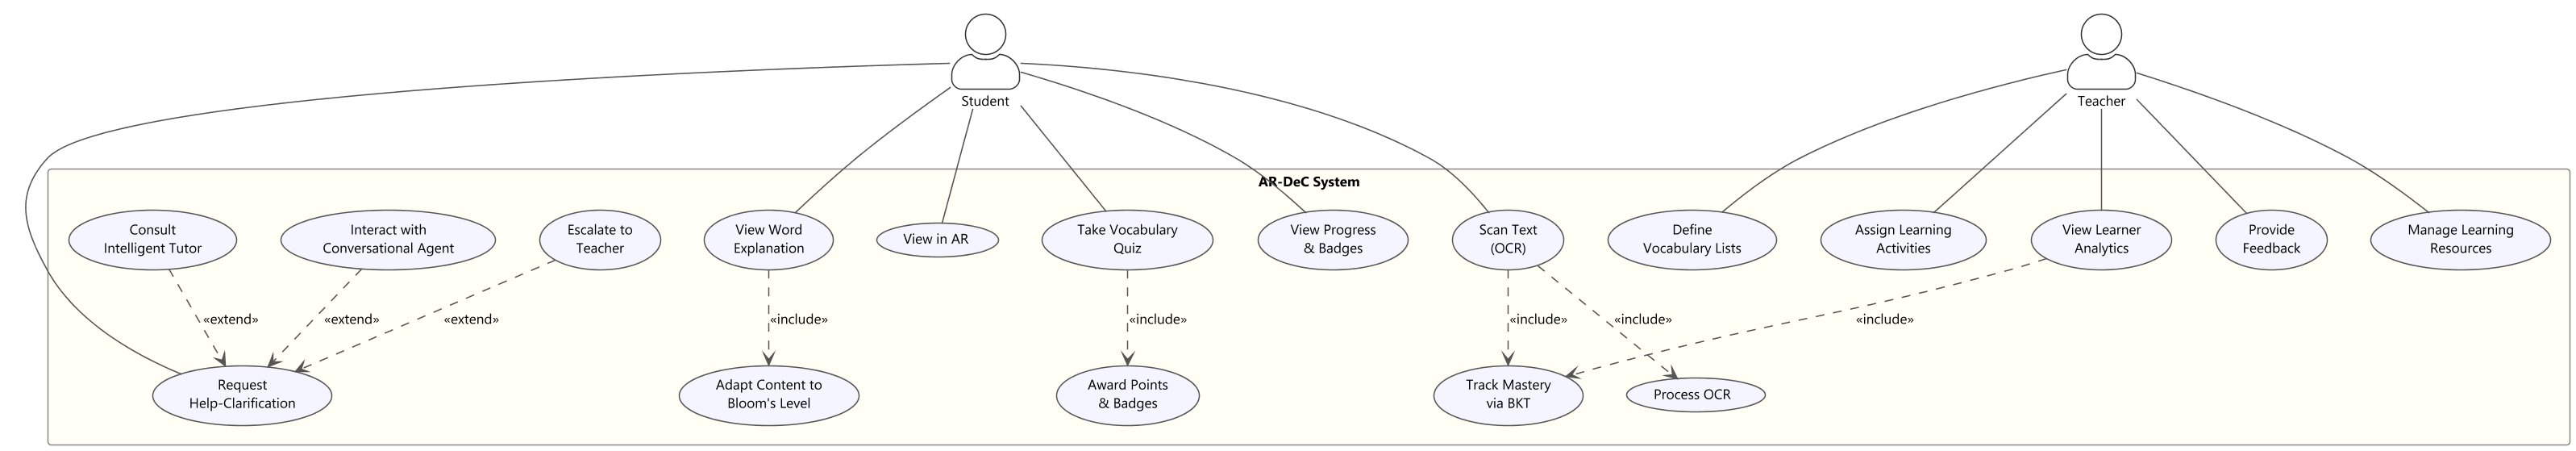
\includegraphics[width=0.9\textwidth,height=0.85\textheight,keepaspectratio]{images/usecase-diagram.png}
\caption{Use case diagram of the AR-DeC system.}
\label{fig:usecase}
\end{figure}

\paragraph{Student use cases.}
The student interacts with the system through six primary use cases. \emph{Scan text} initiates the learning pipeline by capturing a textbook page through the device camera. \emph{View word explanation} allows the student to tap on an extracted word and receive an adaptive, Bloom's-level-calibrated explanation. \emph{View in AR} presents the explanation content as an augmented overlay on the camera feed. \emph{Take vocabulary quiz} engages the learner in a timed, gamified assessment based on recently scanned vocabulary. \emph{View progress and badges} provides a dashboard summarizing the learner's points, level, streak, and earned badges. Finally, \emph{Request help/clarification} triggers a tiered help-seeking mechanism that extends to three sub-use-cases: \emph{Interact with conversational agent} (for quick factual queries), \emph{Consult intelligent tutor} (for in-depth, adaptive explanations), and \emph{Escalate to teacher} (for questions that exceed the system's automated capabilities). This tiered escalation is modeled as an \texttt{<<extend>>} relationship, reflecting the fact that help-seeking is optional and its specific form depends on the nature and complexity of the learner's question.

\paragraph{Teacher use cases.}
The teacher's role encompasses five use cases that collectively ensure pedagogical oversight. \emph{Define vocabulary lists} allows the teacher to curate domain-specific word sets aligned with curricular objectives. \emph{Assign learning activities} enables the creation and distribution of targeted scanning and quiz tasks. \emph{View learner analytics} provides access to aggregated and individual progress data; this use case includes a \emph{Progress tracking} sub-use-case via an \texttt{<<include>>} relationship, reflecting that analytics necessarily involve the retrieval of tracked progress. \emph{Provide feedback} allows direct, personalized teacher-to-student communication when the system's automated responses are insufficient. \emph{Manage learning resources} permits the teacher to create, update, and organize supplementary learning materials within the system.

\paragraph{System use cases.}
The automated system actor is responsible for four background processes that execute in response to student interactions. \emph{Process OCR} is \texttt{<<include>>}-d by the student's \emph{Scan text} use case, reflecting that every scanning action necessarily triggers OCR processing. \emph{Adapt content to Bloom's level} is similarly \texttt{<<include>>}-d by \emph{View word explanation}, ensuring that every explanation request automatically invokes Bloom's-level adaptation via the tutoring engine~\cite{Bloom1956,Krathwohl2002}. \emph{Track mastery via BKT} updates the student model's mastery estimates after each interaction~\cite{Corbett1994}. \emph{Award points and badges} triggers the gamification engine to evaluate point allocations and badge conditions following learning events~\cite{Keller2010,Deterding2011}.

\paragraph{Relationships.}
The \texttt{<<include>>} relationships in this diagram denote mandatory sub-behaviors: scanning always includes OCR processing, and viewing explanations always includes Bloom's adaptation. The \texttt{<<extend>>} relationships, by contrast, model conditional behaviors: help-seeking may or may not escalate to the conversational agent, ITS, or teacher, depending on the learner's needs. This distinction is pedagogically significant---it encodes the design decision that core learning interactions are always fully supported, while help-seeking is adaptive and context-dependent~\cite{Ouariach2026}.

Having specified \emph{what} each actor can do (use cases) and \emph{what} the system is made of (classes), we now transition to the dynamic view, which captures \emph{how} the system behaves over time.

%%% ===================================================================
\subsection{Dynamic View}
\label{sec:dynamic}

The dynamic view complements the static structure by modeling the temporal aspects of the AR-DeC system: the flow of activities during a learning session and the chronological exchange of messages between components. We present an activity diagram that captures the end-to-end workflow and a sequence diagram that details the message-level interactions during a representative scan-learn-quiz cycle.

%%% -------------------------------------------------------------------
\subsubsection{Activity Diagram}
\label{sec:activity}

The activity diagram in \Cref{fig:activity} models the complete workflow of an AR-DeC learning session, from application launch to session termination. It captures the sequential, conditional, and parallel aspects of the learner's journey through the system.

\begin{figure}[p]
\centering
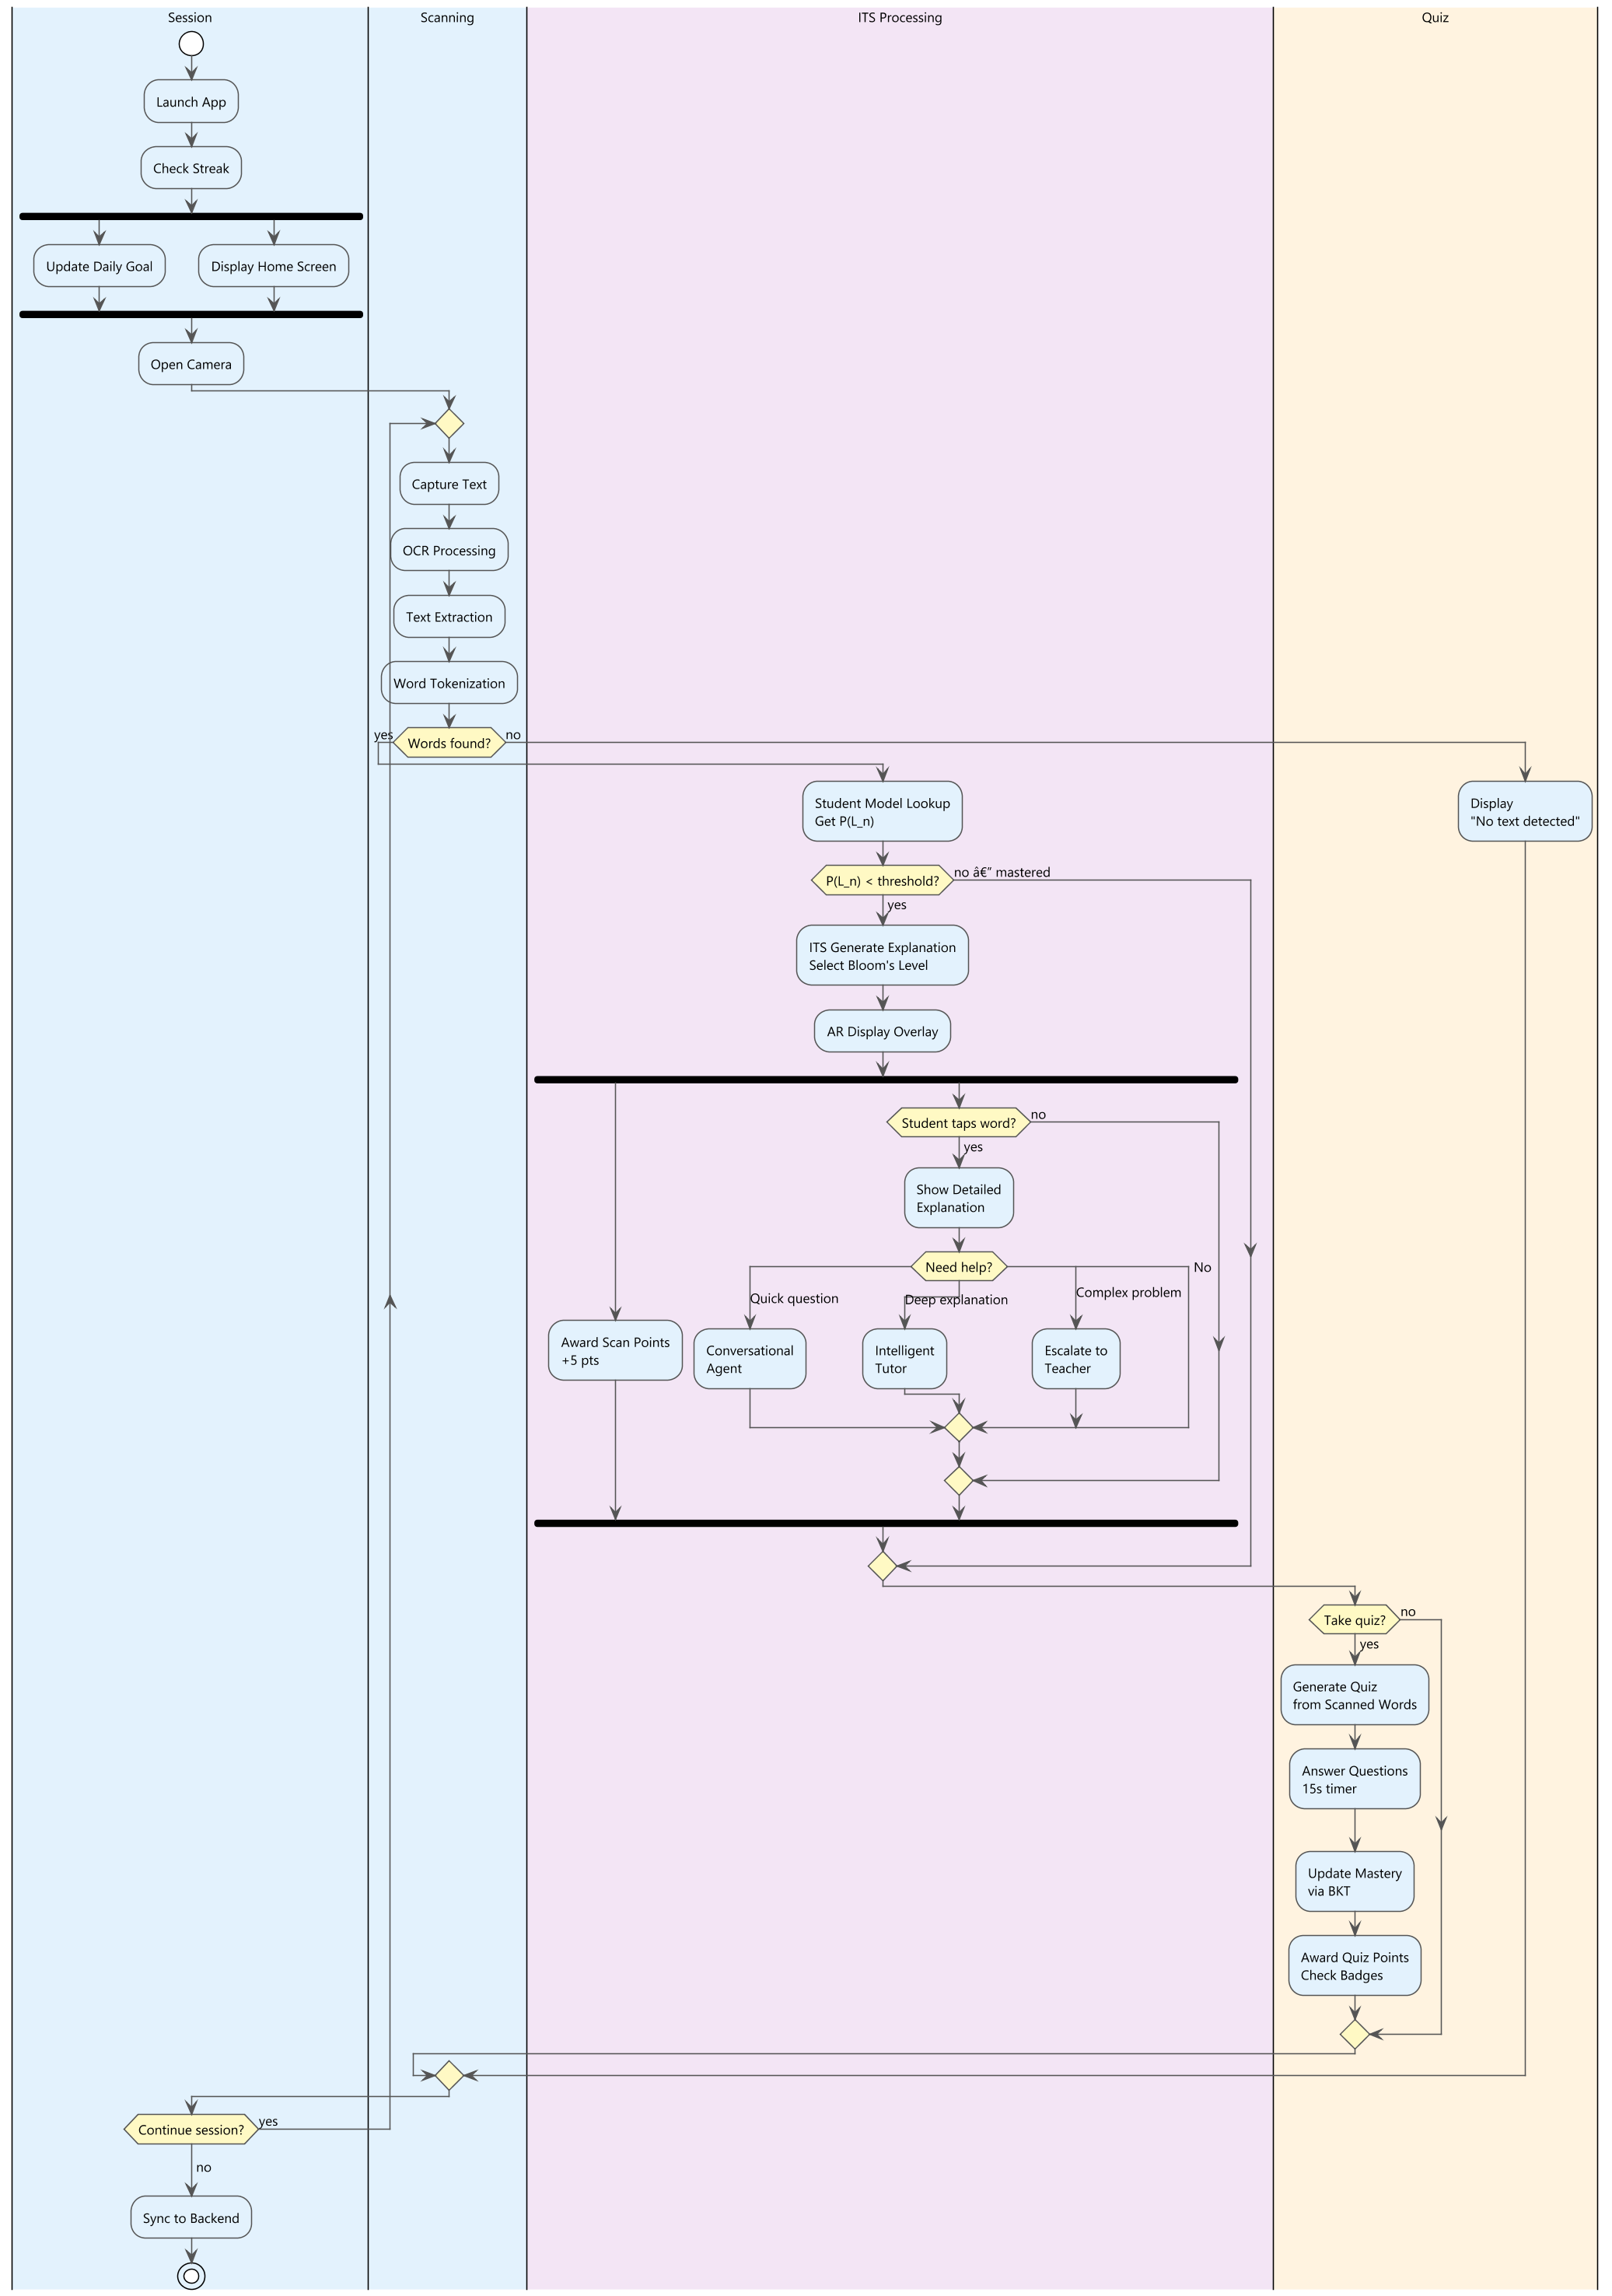
\includegraphics[width=0.85\textwidth,height=0.9\textheight,keepaspectratio]{images/activity-diagram.png}
\caption{Activity diagram of an AR-DeC learning session.}
\label{fig:activity}
\end{figure}

\paragraph{Session start phase.}
The workflow begins with the \emph{Launch application} activity, which triggers a fork into two parallel initialization activities: \emph{Load student profile} and \emph{Check daily streak}. The streak check determines whether the learner has maintained consecutive daily usage, awarding bonus points (+20) if the streak continues or resetting the counter if broken. Once both initialization paths complete (synchronized via a join bar), the system displays the \emph{Home screen}, from which the learner may choose to scan text, take a quiz, or view progress.

\paragraph{Scanning phase.}
If the learner selects the scanning path, the workflow proceeds through \emph{Open camera}, \emph{Capture frame}, \emph{Process OCR} (extracting text from the image), and \emph{Tokenize into words} (segmenting the extracted text into individual \texttt{ScannedWord} instances with bounding box coordinates). A decision diamond evaluates whether words were successfully extracted: if OCR fails (e.g., due to poor image quality or illegible text), the system returns to the camera for a retry; otherwise, the extracted words are passed to the ITS phase.

\paragraph{ITS phase.}
For each selected word, the tutoring engine executes a three-step adaptive process. First, \emph{Look up mastery} queries the \texttt{StudentModel} to retrieve the current $P(L_n)$ for the word~\cite{Corbett1994}. Second, \emph{Select Bloom's level} maps the mastery probability to an appropriate taxonomy stage (e.g., \emph{Remember} for $P(L_n) < 0.3$, \emph{Understand} for $0.3 \leq P(L_n) < 0.6$, \emph{Apply} for $0.6 \leq P(L_n) < 0.8$, \emph{Analyze} for $P(L_n) \geq 0.8$)~\cite{Bloom1956,Krathwohl2002}. Third, \emph{Generate explanation} produces an \texttt{Explanation} object tailored to the selected level, incorporating the word's definition, examples, and related concepts from the \texttt{DomainModel}.

\paragraph{AR display phase.}
The generated explanation is forwarded to the \texttt{ARRenderer}, which executes \emph{Render overlay on camera feed}. A decision diamond determines the rendering mode: \emph{Show definition card} (a floating text panel near the word), \emph{Show 3D model} (a spatial visualization for concepts amenable to three-dimensional representation), or a combination thereof. The learner can interact with the overlay---tapping for more detail, swiping to dismiss, or pinching to resize---before proceeding.

\paragraph{Help-seeking phase.}
At any point during the learning session, the learner may request help, modeled as a decision diamond with three branches. The first branch, \emph{Interact with conversational agent}, handles quick factual queries (e.g., ``What does `photosynthesis' mean?''). A decision diamond evaluates whether the agent's response is sufficient: if yes, the learner returns to the main flow; if no, the request escalates to the second branch, \emph{Consult intelligent tutor}, which provides a deeper, context-aware explanation. If the ITS response is still insufficient, the third branch, \emph{Escalate to teacher}, notifies a human teacher for asynchronous intervention. This tiered escalation ensures that most queries are resolved instantly while reserving human attention for genuinely challenging cases.

\paragraph{Quiz phase.}
The learner may choose to take a vocabulary quiz, triggering \emph{Generate quiz from vocabulary} (which selects questions from recently scanned words, prioritizing those with low mastery). For each question, the learner \emph{Answers within time limit} (15 seconds). A decision diamond evaluates correctness: correct answers trigger \emph{Award points} (+10, multiplied by the combo multiplier for consecutive correct answers) and \emph{Update mastery upward}, while incorrect answers trigger \emph{Show correct answer} and \emph{Update mastery downward}. After all questions, \emph{Calculate final score} produces a summary, and \emph{Check badge conditions} evaluates whether any achievement thresholds have been crossed.

\paragraph{Gamification phase.}
Throughout the session, learning events (scanning, reading, quiz answers) trigger the gamification engine. A fork bar models three parallel activities: \emph{Update points}, \emph{Check and award badges}, and \emph{Update streak counter}. These activities execute concurrently and synchronize at a join bar before \emph{Display gamification feedback} (e.g., a points animation, a badge popup, or a streak notification).

\paragraph{Session end.}
When the learner terminates the session, the system executes \emph{Sync to backend} (persisting the updated student profile, mastery estimates, and gamification state to the Firebase backend) before reaching the final activity node. The decision diamonds throughout the diagram encode the adaptive, learner-driven nature of AR-DeC: the system does not prescribe a rigid path but responds dynamically to the learner's choices and performance.

%%% -------------------------------------------------------------------
\subsubsection{Sequence Diagram}
\label{sec:sequence}

While the activity diagram captures \emph{what happens} during a learning session, the sequence diagram in \Cref{fig:sequence} specifies \emph{who talks to whom and when}---the chronological exchange of messages between the system's key components during a representative scan-learn-quiz cycle.

\begin{figure}[p]
\centering
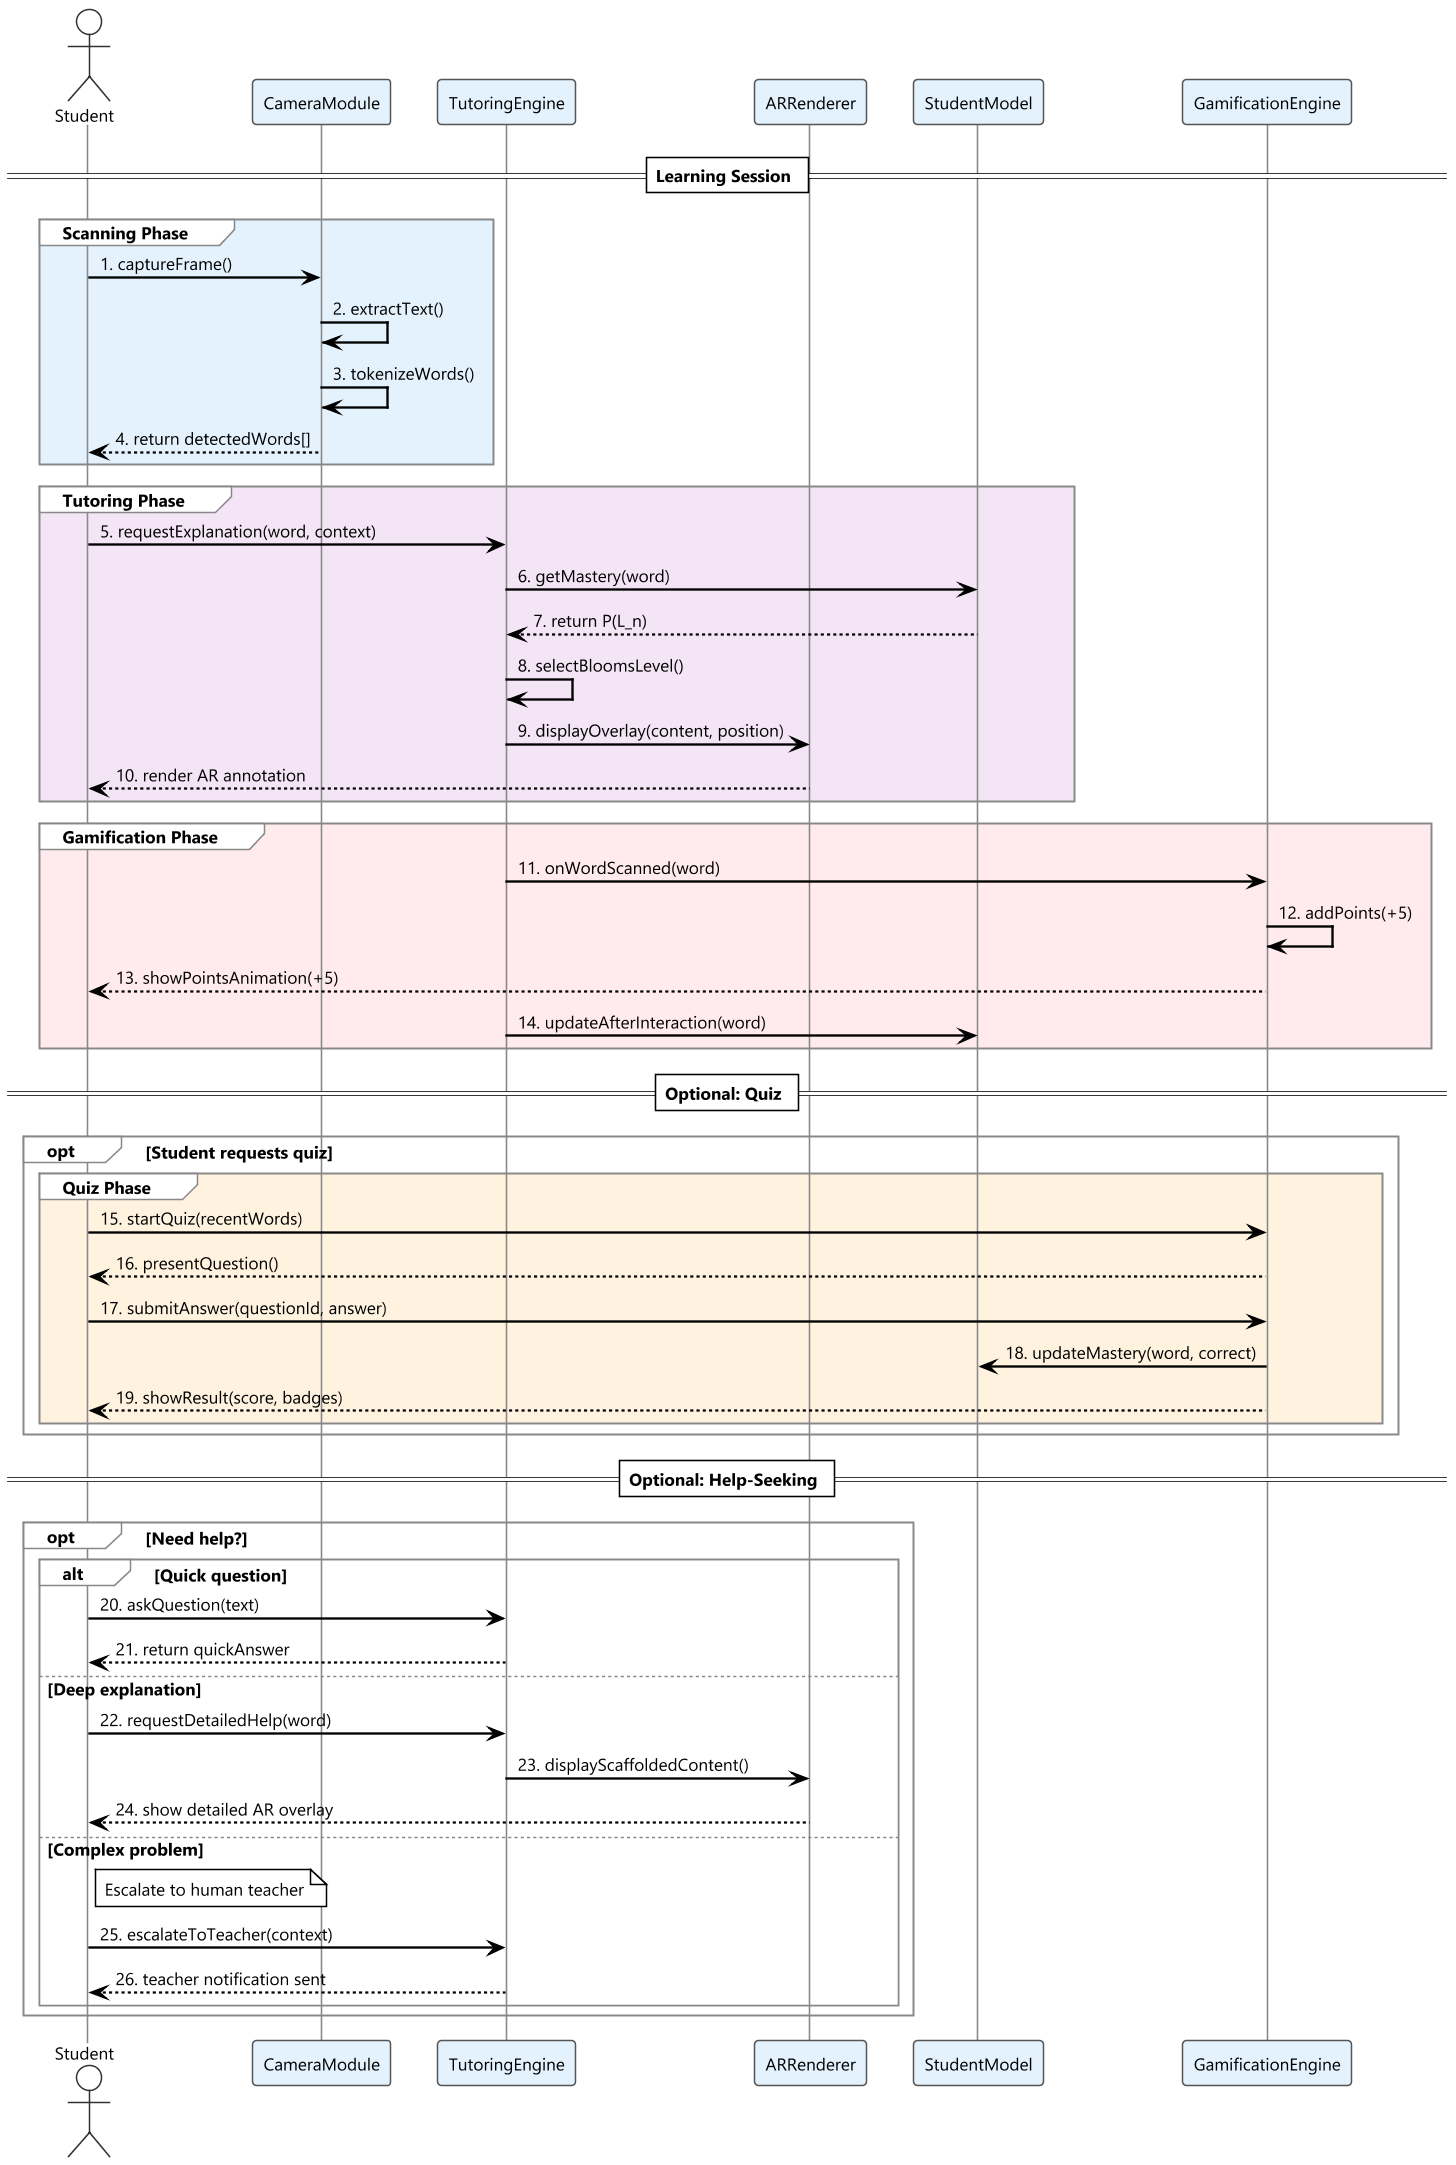
\includegraphics[width=0.85\textwidth,height=0.9\textheight,keepaspectratio]{images/sequence-diagram.png}
\caption{Sequence diagram of a scan-learn-quiz cycle in AR-DeC.}
\label{fig:sequence}
\end{figure}

Six lifelines participate in the interaction: \textbf{Student}, \textbf{CameraModule}, \textbf{TutoringEngine}, \textbf{ARRenderer}, \textbf{StudentModel}, and \textbf{GamificationEngine}. The diagram is organized into three interaction fragments that reflect the modular structure of a learning session.

\paragraph{Main learning session (\texttt{par} fragment).}
The sequence begins when the \texttt{Student} sends a \texttt{scanText()} message to the \texttt{CameraModule}, which responds with an internal \texttt{captureFrame()} call followed by \texttt{extractText()}, returning a list of \texttt{ScannedWord} objects. For each word the student selects (\texttt{selectWord(word)}), the \texttt{CameraModule} forwards a \texttt{getExplanation(word, context)} request to the \texttt{TutoringEngine}. The \texttt{TutoringEngine} queries the \texttt{StudentModel} with \texttt{estimateMastery(word)} to obtain the current $P(L_n)$, computes the appropriate Bloom's level, generates an adapted explanation, and returns it. The explanation is then passed to the \texttt{ARRenderer} via \texttt{displayOverlay(word, position, content)}, which renders the AR visualization and returns a confirmation to the \texttt{Student}. Concurrently, the \texttt{TutoringEngine} sends \texttt{updateAfterInteraction(word, viewed)} to the \texttt{StudentModel} and \texttt{onWordScanned(word)} to the \texttt{GamificationEngine}, which awards points and returns any triggered notifications (e.g., badge earned). This parallel execution within the \texttt{par} fragment reflects the system's ability to update mastery and gamification state simultaneously with AR rendering, minimizing perceived latency.

\paragraph{Quiz (\texttt{opt} fragment).}
If the student elects to take a quiz, a \texttt{takeQuiz()} message initiates an \texttt{opt} (optional) fragment. The \texttt{GamificationEngine} sends \texttt{generateFromVocabulary(recentWords)} to create a quiz, then iterates through questions. For each answer submitted (\texttt{submitAnswer(questionId, answer)}), the \texttt{GamificationEngine} sends \texttt{updateAfterInteraction(word, correct)} to the \texttt{StudentModel} and internally computes the score with combo multipliers. Upon quiz completion, the results are returned to the \texttt{Student}, along with any badges triggered by the \texttt{checkBadges()} evaluation.

\paragraph{Help-seeking (\texttt{opt} fragment with \texttt{alt} conditions).}
A second \texttt{opt} fragment models the help-seeking pathway, activated when the student sends an \texttt{askForHelp(question)} message. An \texttt{alt} (alternatives) combined fragment within this \texttt{opt} specifies three conditions: (1)~if the question is factual, it is routed to the \texttt{ConversationalAgent} (represented as an additional lifeline activated only within this fragment); (2)~if the question requires deeper adaptive explanation, it is routed to the \texttt{TutoringEngine}; (3)~if neither automated component can provide a satisfactory response, the system escalates to the \texttt{Teacher} lifeline via an asynchronous notification. This tiered architecture ensures that the most resource-efficient support channel is always attempted first.

%%% -------------------------------------------------------------------
\subsubsection{Synthesis}
\label{sec:synthesis}

The four UML diagrams presented in this section collectively provide a complete, multi-perspective specification of the AR-DeC pedagogical scenario. The \textbf{class diagram} answers the question of \emph{who} the participants are and \emph{what} they know and can do, establishing the structural vocabulary of the system through fifteen classes with well-defined attributes, methods, and relationships. The \textbf{use case diagram} answers \emph{what each actor can do}, delineating the system boundary and the services available to students, teachers, and automated processes. The \textbf{activity diagram} answers \emph{how the learning flows}, modeling the sequential, conditional, and parallel aspects of an end-to-end learning session. The \textbf{sequence diagram} answers \emph{who talks to whom and when}, specifying the precise chronological message exchange between components during a representative interaction cycle.

Together, these four views ensure traceability from pedagogical intent to technical design: every class can be linked to an educational requirement (e.g., the \texttt{StudentModel} implements BKT~\cite{Corbett1994}), every use case maps to a learner or teacher need, every activity corresponds to a step in the learning process, and every message in the sequence diagram implements a method defined in the class diagram~\cite{Booch2005,Rumbaugh2004}. This traceability is particularly valuable in the context of educational software, where the risk of pedagogical drift---the gradual divergence between educational goals and implemented functionality---is a persistent concern~\cite{Ouariach2023,Ouariach2026}. The UML-driven approach adopted here mitigates this risk by making pedagogical decisions explicit, formal, and verifiable at every level of abstraction.
